% 20200719
\documentclass[../thesis.tex]{subfiles} %% use packages & commands as this main file
\begin{document}
\section{Result}
Biomass densities were stable within days in destructive systems.  \Phy\ biomass densities in both systems dropped during system development (Fig.\ref{f:destCarbon}B).  \Bac\ density had a increase and set back a little to the stable level (Fig.\ref{f:destCarbon}C).  Organic carbon in both systems behaved differently (Fig.\ref{f:destCarbon}A).  It accumulated linearly in \PoN\ but dropped to stability level in \PBN.  Daily yield was significantly different (Fig.\ref{f:ydByHarv}A; p $\ll$ 0.01) between systems or across time except \PoN\ system after the first few days of system development (Fig.\ref{f:ydDaily}A \& \ref{f:ydByHarv}A; p$>$0.1 for \PoN\ day 5 \& 50).  Yield level plateau at long runtime for \phy-only systems but it peaked early in \PBN\ systems (Fig.\ref{f:ydDaily}).  Yet \phy-only systems always had a higher yield distribution than \pbs s with less \phy\ biomass (Fig.\ref{f:destCarbon}B).

Feasible systems in continuous harvest modes had positive yields.  Favourable systems in destructive harvest modes had yields higher than initial values.  85.4\% (n=4695, N=5500; $x$=19500 \dayU; IQR=[0.039, 1.853] \dxdt; median=0.371 \dxdt; max=346 \dxdt) \PoH\ and 0.3\% (n=19; $x$=2101 \dayU; IQR=[0, 0] \dxdt; median=0 \dxdt; max=285 \dxdt) of \PBH\ systems were feasible.  100\% (n=5500; $T$=19900 days; IQR=[0.045, 1.851] \dxdt; median=0.379 \dxdt; max=346 \dxdt) \PoN\ systems and 59.8\% (n=3288; $T$=91 days; IQR=[-0.015, 0.119] \dxdt; median=0.013 \dxdt; max=243 \dxdt) \PBN\ systems were favourable.  Most system pairs showed significance in median difference (\PoH\ vs \PoN: p=0.36; other pairs: p$\ll$0.01).  \Bac l invasion into \PoN\ systems hence would have around 60\% chance of maintaining a fraction of its expected function (Fig.\ref{f:bacEffect}).  With the right combination of \phy\ and \bac, \pbs s could also have yield comparable with \phy-only systems.

Most \phy\ biology had significant (p$\ll$0.01 for Wilcox test across the ends of parameter ranges) unidirectional ($\ePR$, $\eP$, $\gP$: positive; $\aP$: negative) effect on log yield distributions (Fig.\ref{f:bacEffect}).  \Bac\ biology had no observable distribution influences (Fig.\ref{f:bacEffect2}).  Harvest modes determined feasibility of \pbs s (Fig.\ref{f:harvPB}) but had no effect on \phy-only systems (Fig.\ref{f:harvPo}).  In short, yield distribution maximized when \phy\ had high carbon-to-biomass ratio (high $\ePR$ and $\eP$), high growth rate (high $\gP$) and low intraspecific interference (low $\aP$).

\begin{figure}[H]
    \centering
    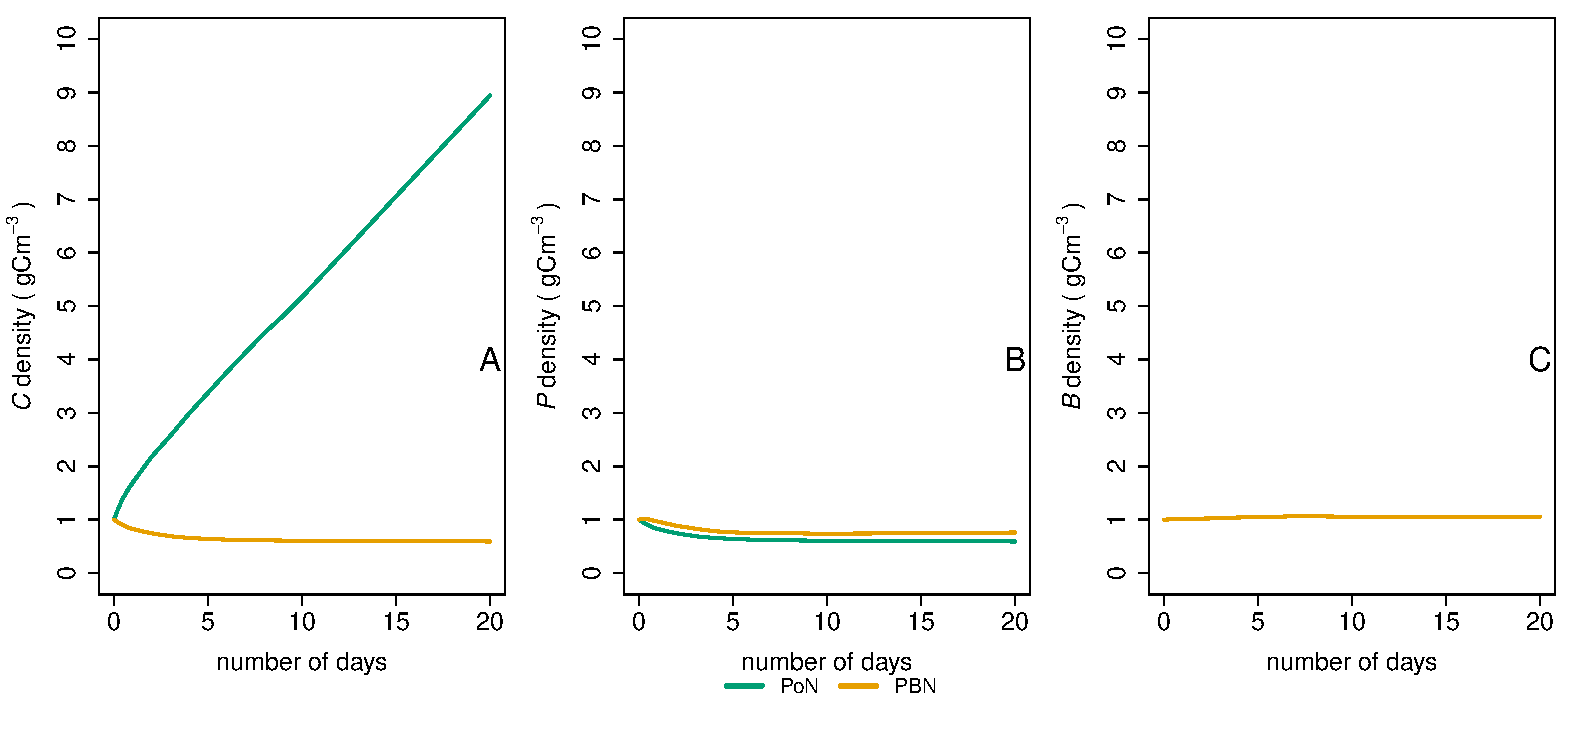
\includegraphics[width=\linewidth]{result/Sample.pdf}
    \caption[Median carbon content in destructive systems]{Median carbon content in destructive systems.  $C$, $P$ and $B$ were carbon pools in Fig.\ref{f:model}.  Eq.\ref{eq:PBH} was used with different initial carbon densities to address the \PoN\ and \PBN\ modes.  Initial carbon densities for \PoN\ were [1,1,0]\den\ ($C$, $P$, $B$) and that for \PBN\ were [1,1,1]\den.  Note that both systems had similar levels of \phy\ across time \textbf{(B)}.  Yet due to the presence of \bac\ \textbf{(C)}, organic carbon pool density changes were huge \textbf{(A)}.  Also note that after a initial boost, accumulation of organic carbon was linear for \PoN\ \textbf{(A)}.  Note that existence of \bac\ suppressed the organic carbon density in the system \textbf{(A)} with almost unchanged \bac\ biomass density \textbf{(C)}.}
    \label{f:destCarbon}
\end{figure}

\begin{figure}[H]
    \centering
    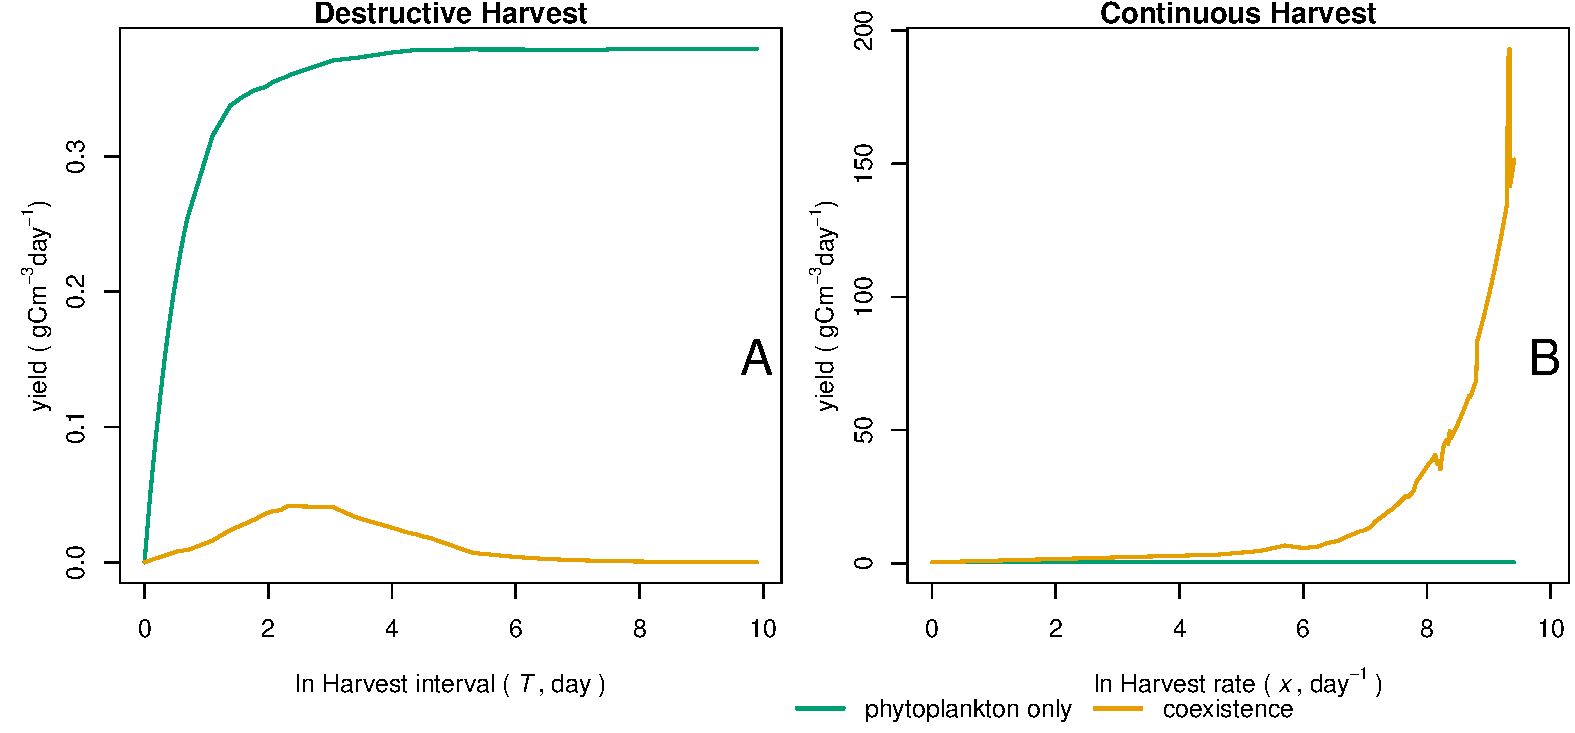
\includegraphics[width=\linewidth]{result/DailyYield.pdf}
    \caption[Median daily yield across systems]{Median daily yield across systems.  Note that both harvest interval/rate were natural logged to emphasize daily yield changes when carbon was harvested more frequent \textbf{(A)} or less amount \textbf{(B)}.  Also note that lower part of \textbf{(B)} was empty because we did not collect such fine-scaled data.  In plot \textbf{A}, the minimal optimum harvest interval for \PoN\ was around 55 days (i.e. exp(4)) while peak yield achieved at day 20 (i.e. exp(3)) for \PBN.  For continuous harvest \textbf{(B)}, very high daily harvest destabilised \PoH\ systems.  Yet for majority of \PBH\ systems, daily yield was zero because such system only feasible for a tiny portion (0.3\%) of the 1.1 million simulated scenarios.}
    \label{f:ydDaily}
\end{figure}

\begin{figure}[H]
    \centering
    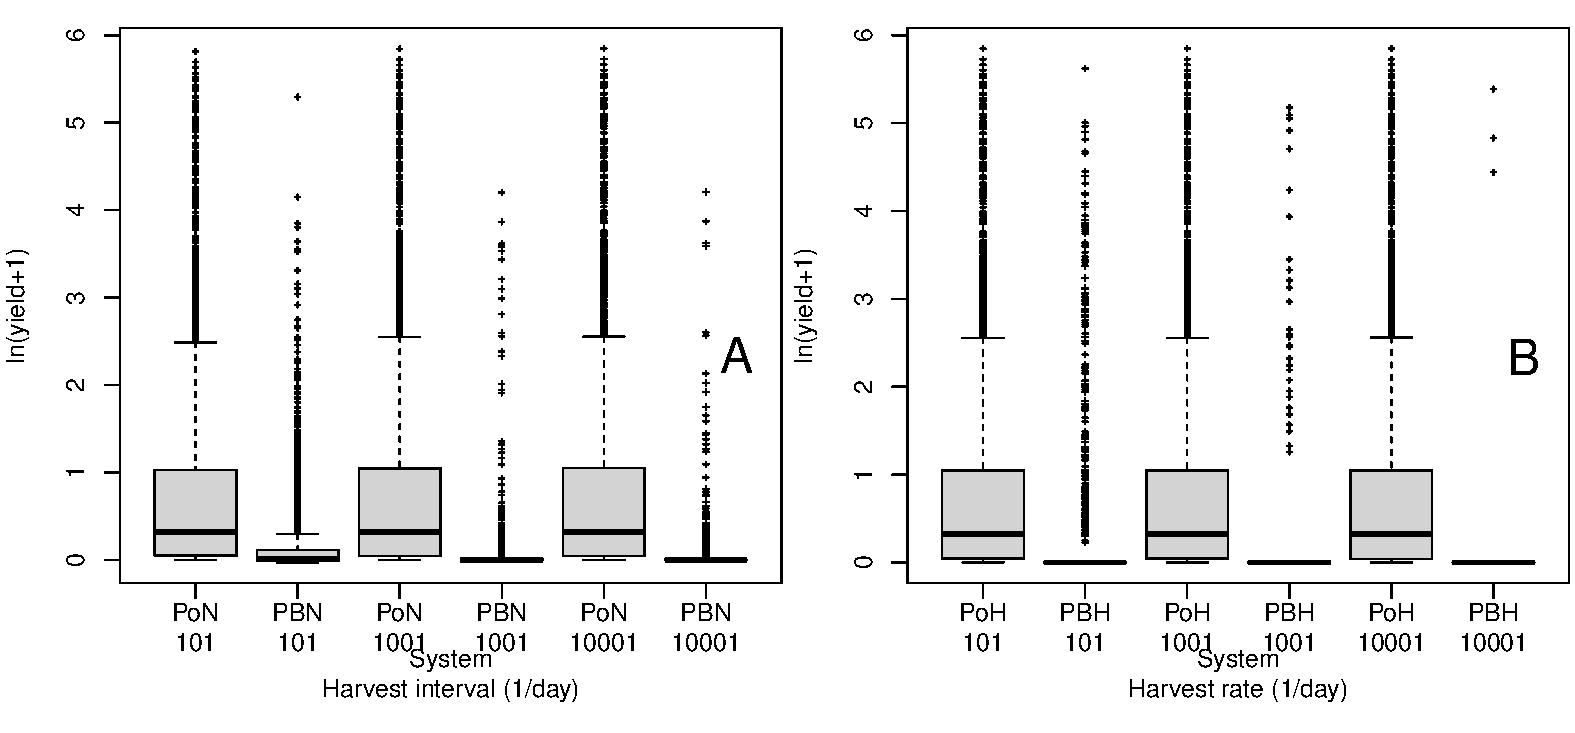
\includegraphics[width=\linewidth]{result/Harvest.pdf}
    \caption[Yield flux distribution by harvest mode]{Log distribution of yield for destructive \textbf{(A)} and continuous \textbf{(B)} harvest modes on selected harvest interval/rates.  \textbf{(A)} Pairwise Wilcox test showed significance (p $\ll$ 0.01) between all except the pair of \PoN\ systems interval 5 and 50 days (p $>$ 0.1).  For \PBN\ systems 0.5 days harvest interval, some systems recorded an initial drop of organic carbon and caused a slight negative yield (none of the drops exhausted the initial organic carbon pool).  The drop recovered in later time with a large variation in yield recovery.  \textbf{(B)} \PoH\ and \PBH\ systems were significantly different (p $\ll$ 0.01).  Significance was also found between \pbs s (p $\ll$ 0.01) but not \phy-only systems (p $>$ 0.1).  Each box represented a sample size of 5500.}
    \label{f:ydByHarv}
\end{figure}

\begin{figure}[H]
    \centering
    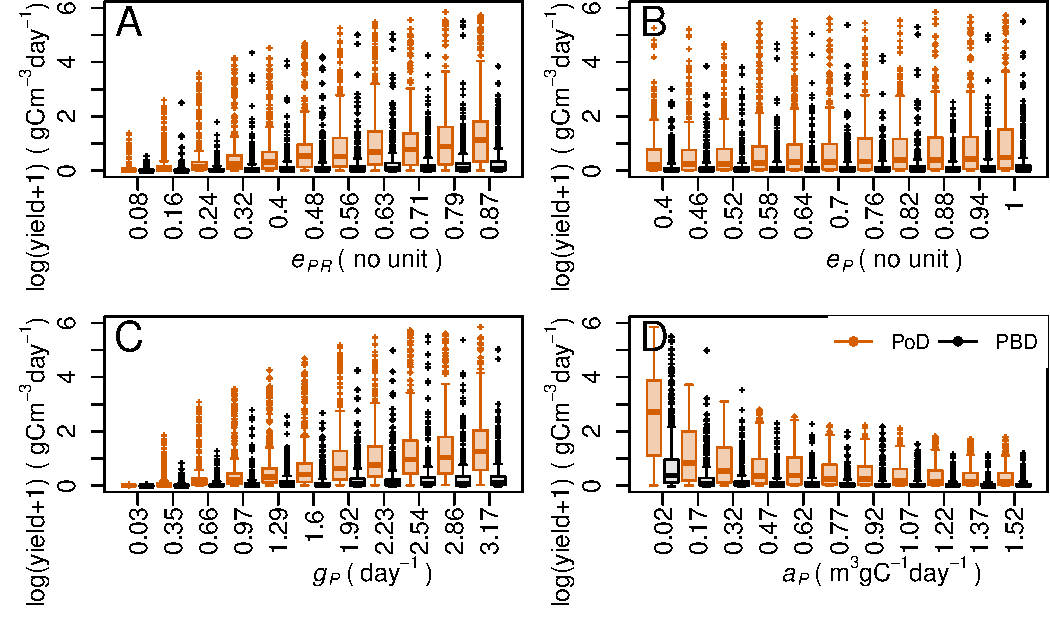
\includegraphics[width=\linewidth]{result/bacEff1.pdf}
    \caption[Log yield flux comparisons between \phy-only and \pbs s on \phy\ parameters]{Log yield flux comparisons between \phy-only and \pbs s on \phy\ parameters.  Full description of variables were in Table \ref{t:ranges}.  Each group in each plot had an LHS sample size of 5500.  Pairwise Wilcox test showed significance (all p $\ll$ 0.01) between the systems and the ends of parameter ranges.  Note that only a few scenarios of \pbs s were positives, which symbolised small feasibility.  Also note that ranges of both groups were similar, symbolising comparable yield values were possible for \pbs s when biologically compatible candidates were selected.}
    \label{f:bacEffect}
\end{figure}

\end{document}